\documentclass[hidelinks]{report}

\usepackage[utf8]{inputenc} % Character encoding
\usepackage[english]{babel} % Language

\usepackage[table,xcdraw]{xcolor} % Table colors
\usepackage{tabularx} % Dynamic table width
\usepackage{tcolorbox} % Gray boxes
\usepackage{hyperref} % URL environment
\usepackage{todonotes} % Notes
\usepackage{natbib} % Bibliography
\usepackage{fancyhdr} % Header and footer
\usepackage{multirow} % Multirow
\usepackage{geometry} % Page layout
\usepackage{color} % Text colors
\usepackage{float} % Show tables within their section
\usepackage{listings} % Code
\usepackage{pdflscape} % Horizontal orientation (landscape)
\usepackage{enumerate} % Custom enumerators

% Command for inline code
\newcommand{\code}[1]{\lstinline[language=json,columns=fixed,breakatwhitespace]{#1}}

% Commands for requirements priorities
\newcommand{\priohigh}{1 - high}
\newcommand{\prioavg}{2 - average}
\newcommand{\priolow}{3 - low}
\newcommand{\prioopt}{4 - optional}

% JSON display
\colorlet{punct}{red!60!black}
\definecolor{background}{HTML}{EEEEEE}
\definecolor{delim}{RGB}{20,105,176}
\colorlet{numb}{magenta!60!black}

\lstdefinelanguage{json}{
    basicstyle=\normalfont\ttfamily,
    numbers=left,
    numberstyle=\scriptsize,
    stepnumber=1,
    numbersep=8pt,
    showstringspaces=false,
    breaklines=true,
    frame=lines,
    backgroundcolor=\color{background},
    literate=
     *{0}{{{\color{numb}0}}}{1}
      {1}{{{\color{numb}1}}}{1}
      {2}{{{\color{numb}2}}}{1}
      {3}{{{\color{numb}3}}}{1}
      {4}{{{\color{numb}4}}}{1}
      {5}{{{\color{numb}5}}}{1}
      {6}{{{\color{numb}6}}}{1}
      {7}{{{\color{numb}7}}}{1}
      {8}{{{\color{numb}8}}}{1}
      {9}{{{\color{numb}9}}}{1}
      {:}{{{\color{punct}{:}}}}{1}
      {,}{{{\color{punct}{,}}}}{1}
      {\{}{{{\color{delim}{\{}}}}{1}
      {\}}{{{\color{delim}{\}}}}}{1}
      {[}{{{\color{delim}{[}}}}{1}
      {]}{{{\color{delim}{]}}}}{1},
}

% Cucumber.
\lstdefinelanguage{Gherkin}{
  keywords={When, Then, Given, And},
  ndkeywords={Feature, Scenario},
  sensitive=true,
  comment=[l]{!--},
  morestring=[b]"
}

% Configure page layout
% Page layout
\geometry{
	bottom=3.5cm,
	headheight=180pt
}

% Nummerierung der ersten Seiten verhindern
\pagenumbering{gobble}

% Bibstyle
\bibliographystyle{plain}

% Header / Footer
\fancypagestyle{plain}{
	\fancyhf{}% Clear header/footer
	\fancyhead[R]{
\includegraphics[width=4cm]{img/aa-logo}} % Rechter header
	\fancyhead[L]{\leftmark} % Linker header
	\fancyfoot[R]{\thepage} % Rechter footer
}
\pagestyle{plain}

\renewcommand{\headrulewidth}{0.5pt} % Unnötige Informationen der Kapitelangabe
\renewcommand{\footrulewidth}{0.2pt} % entfernen
\renewcommand{\chaptermark}[1]{\markboth{{#1}}{}}

% Zahlen für Fußnoten
\renewcommand{\thefootnote}{\arabic{footnote}}
\renewcommand{\thempfootnote}{\arabic{mpfootnote}}


% Title page
% Document name
\newcommand{\documentname}{Technical documentation}
\newcommand{\documentVersion}{2.0}

% Project name
\newcommand{\projectNameShort}{VRGP}
\newcommand{\projectNameLong}{VRGP implementation for the Åboat}
\newcommand{\projectName}{{\projectNameLong} (\projectNameShort)}

% Course name
\newcommand{\course}{Project course}
\newcommand{\semester}{2021 - 2022}

% Gruppenmitgieder.
\makeatletter
\newcommand{\memberOne}   {Md Hredoy Mesha & \href{mailto:meshahredoy@gmail.com}{meshahredoy@gmail.com}}
\newcommand{\memberTwo}   {Gabriela Corbalan Gomez & \href{mailto:gabri.corba@gmail.com}{gabri.corba@gmail.com}}
\newcommand{\memberThree} {Daniel Gonzálves Alfert & \href{mailto:danielgalfert@gmail.com}{danielgalfert@gmail.com}}
\newcommand{\memberFour}  {Alexandru Gherghescu & \href{mailto:alexandru.gherghescu@abo.fi}{alexandru.gherghescu@abo.fi}}
\newcommand{\memberFive}  {Joan Dolz Mensua & \href{mailto:joan.dolzmensua@abo.fi}{joan.dolzmensua@abo.fi}}
\newcommand{\memberSix}   {Elijah Rose & \href{mailto:elijah.rose@abo.fi}{elijah.rose@abo.fi}}
\newcommand{\memberSeven} {Yannick Zapfe & \href{mailto:yannick.zapfe@abo.fi}{yannick.zapfe@abo.fi}}
\makeatother

\title{
	\vspace*{-3cm}
	\projectName\\
	\documentname\\
	Version \documentVersion\\
	-\\
	\color{gray}
	\course\ \semester\\
	\vspace*{5mm}
	
\includegraphics[width=0.5\textwidth]{img/vrgp-logo}
}

\author{
	\begin{tabular}{r l@{\hspace{7\tabcolsep}} r}
		\memberOne   \\
		\memberTwo   \\
		\memberThree \\
		\memberFour  \\
		\memberFive  \\
		\memberSix   \\
		\memberSeven
	\end{tabular}
}

\date{\today}


% Document

\begin{document}
	\maketitle
	
	\chapter*{Revision history}
	
	\begin{table}[H]
		\centering
		\begin{tabularx}{\textwidth}{ l c X }
			\rowcolor[HTML]{C0C0C0}
			\textbf{Date} & \textbf{Version} & \textbf{Description} \\
			07.10.2021 & 1.0   & Initial version \\
			\rowcolor[HTML]{E7E7E7}
			21.10.2021 & 1.1   & Roles refinement, schedule update \\
			26.10.2021 & 1.2.1 & Update resources and budget \\
			\rowcolor[HTML]{E7E7E7}
			26.10.2021 & 1.2.2 & Update schedule \\
			29.10.2021 & 1.2.3 & Update project organisation: Add developer role \\
			\rowcolor[HTML]{E7E7E7}
			05.11.2021 & 1.3   & Make changes according to feedback session \\
			07.11.2021 & 1.4   & Update activities chapter and refine project vision \\
			\rowcolor[HTML]{E7E7E7}
			17.11.2021 & 1.5   & Translation to LaTeX \\
		\end{tabularx}
	\end{table}
	
	\tableofcontents
	
	\chapter{Project overview}\label{chp:overview}
	\pagenumbering{arabic} % Start page numbering.
	\thispagestyle{fancy}
	\section{Product vision statement}\label{sec:vision}

Our vision is to provide software that ensures the safe navigation of possibly autonomous ships by implementing the vessel side of the Vessel Remote Guidance Protocol (VRGP). We aim to show that the protocol works by providing a prototype implementation for the Åboat with a generic core implementation of the protocol that can be used as a starting point for real-world implementations.
\\\\
The goal of the VRGP protocol is for vessels to securely communicate in real-time with on-shore maritime operating centers (MOC) which can provide guidance, e.g. for docking vessels. Ultimately, this would avoid putting lives in danger when docking vessels as the physical presence on-board would become unnecessary. The protocol allows access to key sensors and even video data on vessels to provide MOCs with relevant up-to-date information.
\\\\
We envision future use of the protocol for autonomous boats. Via the protocol, they could receive guidance from different MOCs along the way from one harbour to another. The protocol is specified such that only requested information is sent over the network. This would reduce network latency and bandwidth consumption.
\\\\
As this is supposed to include a standard implementation of the protocol, shipping companies will need to adjust it to real-world applications. With that in mind, this implementation has to be easily integratable into already running systems.

\section{Project deliverables}\label{sec:deliverables}

The deliverables specific to this project are:

\begin{itemize}
	\item A Docker container with an OpenDLV microservice implementing the vessel-side of the VRGP for the Åboat
	\item An extension of the Åboat user interface to control parts of the VRGP implementation
	\item Improved testing environment, especially including a test implementation of an MOC
	\item Protocol specification contributions
\end{itemize}

\noindent
The additional deliverables required by the course are:

\begin{itemize}
	\item Project plan
	\item Technical documentation
	\item Prototype
	\item User guide
	\item Business plan
	\item Poster
	\item Retrospective analysis
	\item Source code
\end{itemize}

\section{Budget and resources}\label{sec:budget}

\begin{table}[H]
	\centering
	\begin{tabularx}{\textwidth}{ l l X }
		\textbf{Resource} & \textbf{Budget} & \textbf{Description} \\
		\rowcolor[HTML]{C0C0C0}
		\textbf{Hardware} & & \\
		Laptops and computers & €0 & Our own \\
		\rowcolor[HTML]{E7E7E7}
		ICE servers (hosting) & €3-5 per month & Optional/provided by client \\
		Raspberry Pi & €0 & Provided by client \\
		\rowcolor[HTML]{C0C0C0}
		\textbf{Software and tools} & & \\
		GitHub & €0 & Open-source \\
		\rowcolor[HTML]{E7E7E7}
		JavaScript & €0 & Free \\
		C++ & €0 & Free \\
		\rowcolor[HTML]{E7E7E7}
		OpenDLV & €0 & Open-source \\
		Postman & €0 & Free \\
		\rowcolor[HTML]{E7E7E7}
		Microsoft Office & €0 & Provided by university \\
		Zoom & €0 & Provided by university \\
		\rowcolor[HTML]{E7E7E7}
		Discord & €0 & Free \\
		\rowcolor[HTML]{C0C0C0}
		\textbf{Additional tools} & & \\
		Human resources & €0 & No wages \\
		\rowcolor[HTML]{E7E7E7}
		Workspace & €0 & Provided by university \\
		\rowcolor[HTML]{C0C0C0}
		\textbf{Overall budget} & €3-5 per month & \\
	\end{tabularx}
	\label{table:f-req-1}
\end{table}

	
	\chapter{Project organisation}\label{chp:organisation}
	\thispagestyle{fancy}
	As we have a big team, everyone has a specific role and certain responsibilities matching their skills, experience, and interests. We decided on the following roles and preliminary distribution of tasks:

\begin{itemize}
	\item \textbf{Project manager: Hredoy Mesha} \\
		The project manager is, in accordance with the definition in this project course, in charge of organizing the collaboration within the team, including distribution of tasks, keeping an overview of the project progress and deadlines, and team building events.
		\begin{itemize}
			\item Meeting organization and moderation
			\item Make sure everyone is following the deadlines
			\item Keep an overview of the project status
			\item Task supervision
			\item In charge of team happiness (organizing team events)
		\end{itemize}
	\item \textbf{Product owner: Alexandru Gherghescu} \\
		As defined in the course and the Scrum framework, the product owner is responsible for the software product and keeps an overview of the different, possibly parallel software design and development tasks.
		\begin{itemize}
			\item Make sure implementation respects the requirements
			\item Manage the design and architecture of the system
			\item Define, prioritize and adjust implementation-related tasks
			\item Manage the backlog of the project
		\end{itemize}
	\item \textbf{Scrum master: Gabriela Corbalan Gomez} \\
		The Scrum master, another role from the Scrum framework, is in charge of planning the sprints, creating and maintaining the backlog of tasks, and distributing the concrete tasks among the developers.
		\begin{itemize}
			\item Scrum toolchain and workflow
			\item Coach team members
			\item Assist product owner with the backlog of the project
		\end{itemize}
	\item \textbf{Quality manager: Daniel Gonzálvez Alfert} \\
		The quality manager ensures the quality of the software product, in the sense that the code itself is of high quality, by implementing appropriate quality assurance tools.
		\begin{itemize}
			\item Testing toolchain
			\item Make sure code meets quality requirements
			\item Keep track of error logs (problems that arise and solutions to them)
			\item Make sure developers follow the quality standards
			\item Performance checks
		\end{itemize}
	\item \textbf{Security manager: Joan Dolz Mensua} \\
		As we are working on a possibly, and at least theoretically, safety-critical software, the security manager is responsible for the software to be secure and safe.
		\begin{itemize}
			\item Make sure external software interaction is secure
			\item Make sure the implementation on top of the existing software stack is implemented correctly (from a security standpoint)
		\end{itemize}
	\item \textbf{Technical manager: Elijah Rose} \\
		The technical manager ensures a good workflow for the team by setting up and maintaining several tools for communication and collaboration including work on the documentation as well as the actual software.
		\begin{itemize}
			\item Maintain coding tools coherency
			\item Make sure people respect the conventions adopted in the tools used by the team
			\item Head developer
			\item Coding tasks distribution
		\end{itemize}
	\item \textbf{Documentation manager: Yannick Zapfe} \\
		The documentation manager is in charge of the documentation of the software product, starting with the requirements documentation and including the design documentation and finally the software documentation and the user guide.
		\begin{itemize}
			\item Communication with the client
			\item Make sure code is well documented and documentation is up-to-date
			\item Make sure technical and user documentation is up-to-date
		\end{itemize}
	\item \textbf{Developers: Alexandru, Gabriela,  Daniel,  Joan, Yannick, and Elijah} \\
		Except for the project manager, each team member was, in addition, also involved in the software development process as a developer or tester.
\end{itemize}

\noindent
The project has two customers belonging to two different organizations:

\begin{itemize}
	\item \textbf{Robert Aarts (Aboa Mare)} \\
		Aboa Mare provides the protocol specification as well as a rudimentary implementation of and testing environment for the protocol.
	\item \textbf{Kai Jämsä (Åboat)} \\
		Åboat is the target environment for the software product to work in. Kai Jämsä from Åboat provides the project with the technical necessities and knowledge for us to build a working software product.
\end{itemize}

	
	\chapter{Activities and milestones}\label{chp:activities}
	\thispagestyle{fancy}
	\section{Activities}\label{sec:activities}

There are many activities to be considered that are important for the completion of this project. As we are working on potentially safety-critical software, we need to have a thorough understanding of the requirements and a solid design to base our implementation on. To ensure that the requirements specification matches the actual needs of our customers and that our software design and architecture supports the correct implementation of these requirements, we will continuously update and refine the requirements and the design. Another important part of our project is the quality assurance process which helps us check our own work constantly throughout the project.

\subsection{Technical feasibility analysis}\label{sec:feasibility}

As the Åboat software project is already implemented as a microservice architecture, we are sure that the VRGP implementation will be able to run within the existing software environment of the Åboat. Basically, it means adding another microservice - as a Docker container - which runs the vessel-side VRGP implementation and communicates with the other microservices, especially those that provide the sensor data of the Åboat. No, or very minimal, additional hardware, which would be provided by the Åboat project, needs to be added to support the VRGP implementation on the Åboat.
\\\\
A minimal proof of concept for the VRGP protocol also already exists in the form of a simple MOC test implementation (available on \href{https://github.com/RemoteBoatX/vrgp-docs/tree/main/moc-environment}{GitHub}) which communicates with a mobile device, simulating a vessel in this context. The mobile device can transmit very basic information: network time, response latency, and basic video output. This prototype implementation is by AboaMare.

\subsection{Requirement analysis}\label{sec:requirements}

In the initial phase of the project, we stayed in regular and close contact to our customers to acquire a thorough understanding of the requirements and to formulate these initial requirements as the basic pillar for the design of the system. These requirements were continuously reassessed and refined over the course of the project.
\\\\
We agreed with our customers to split the system into a maximum of ten high-level functional requirements which are refined by sub-requirements. This ensures that the requirements can be easily understood even by persons not familiar with the technicalities of the project. It also lays a foundation for the design of the software.
\\\\
The requirements can be found in the technical documentation of this project.

\subsection{Design}\label{sec:design}

The software design and architecture is based on the requirements, as described in the previous section. Like the requirements, the design was reassessed and refined throughout the project. While the requirements were negotiated and closely coordinated with the customers, most of the software design and architecture within the given software environment were up to us. The boundaries that are set by the existing software environment are:

\begin{itemize}
	\item The VRGP implementation for the Åboat runs as a microservice or a set of microservices within a microservice architecture.
	\item The microservice is deployed as an independent Docker container.
	\item The microservice communicates with other microservices within the Åboat software environment.
	\item The existing MOC test implementation by AboaMare can serve partly as a guide for our MOC prototype.
\end{itemize}

\subsection{Implementation}\label{sec:implementation}

Following the initial design phase and based on the software design and architecture, we began implementing the actual system.
\\\\
As there are already systems present on the Åboat that we needed to interface with, we had an initial technology stack already in place, which we had to build upon. This consists of the following technologies already present:

\begin{itemize}
	\item OpenDLV (main framework for communication between microservices)
	\item C++ as a server and interfacing language
	\item Docker as a container solution
	\item JavaScript was used to build the existing prototype for the Maritime Operating Center
\end{itemize}

\noindent
Additional tools and technologies were needed through the project, to test, implement or otherwise help with the codebase. These included tools like:

\begin{itemize}
	\item JenkinsCI (for building and monitoring)
	\item Postman (for API testing and interaction)
	\item Additional languages for easier prototyping (Python)
\end{itemize}

\noindent
The implementation of the system can be split into the following major tasks, which were extended over the course of the project:

\begin{itemize}
	\item Developing the software in an independent container capable of interacting with the other parts of the system.
	\item Creating the necessary network and communication infrastructure.
	\item Implementing the vessel side of the VRGP protocol.
	\item Testing the communication between a mock-up MOC and the vessel.
\end{itemize}

\subsection{Quality assurance}\label{sec:quality}

Over the course of the project, beginning with the initial requirements analysis phase, we had quality assurance measures in place to ensure a safe and high-quality software product. An important part of this process was the regular meetings with our customers as well as peer and team reviews within our project team.
\\\\
With the beginning of the implementation phase, we conducted software quality checks with every feature added or piece of code changed. This includes:

\begin{itemize}
	\item Continuous testing and integration
	\item Continuous deployment and application building
	\item Security checks
	\item Quality assurance of the final product
\end{itemize}

\noindent
This way there was a continuous tracking of the product quality. Throughout the project, we also made sure that the features which are being developed respect the requirements agreed upon with the customers. If any requirements changed, we adapted the software accordingly.
\\\\
Following the prototyping phase of the project, we also used monitoring tools to ensure the proper functioning of both the server and the client-side software.

\section{Tasks, milestones and schedule}\label{sec:schedule}

The schedule is rather detailed by now, but is reevaluated and adjusted every week in our team meetings. The planned phases, especially those that lie further in the future, are estimated and subject to change over the course of the project.

\begin{figure}[ht]
	\centering
	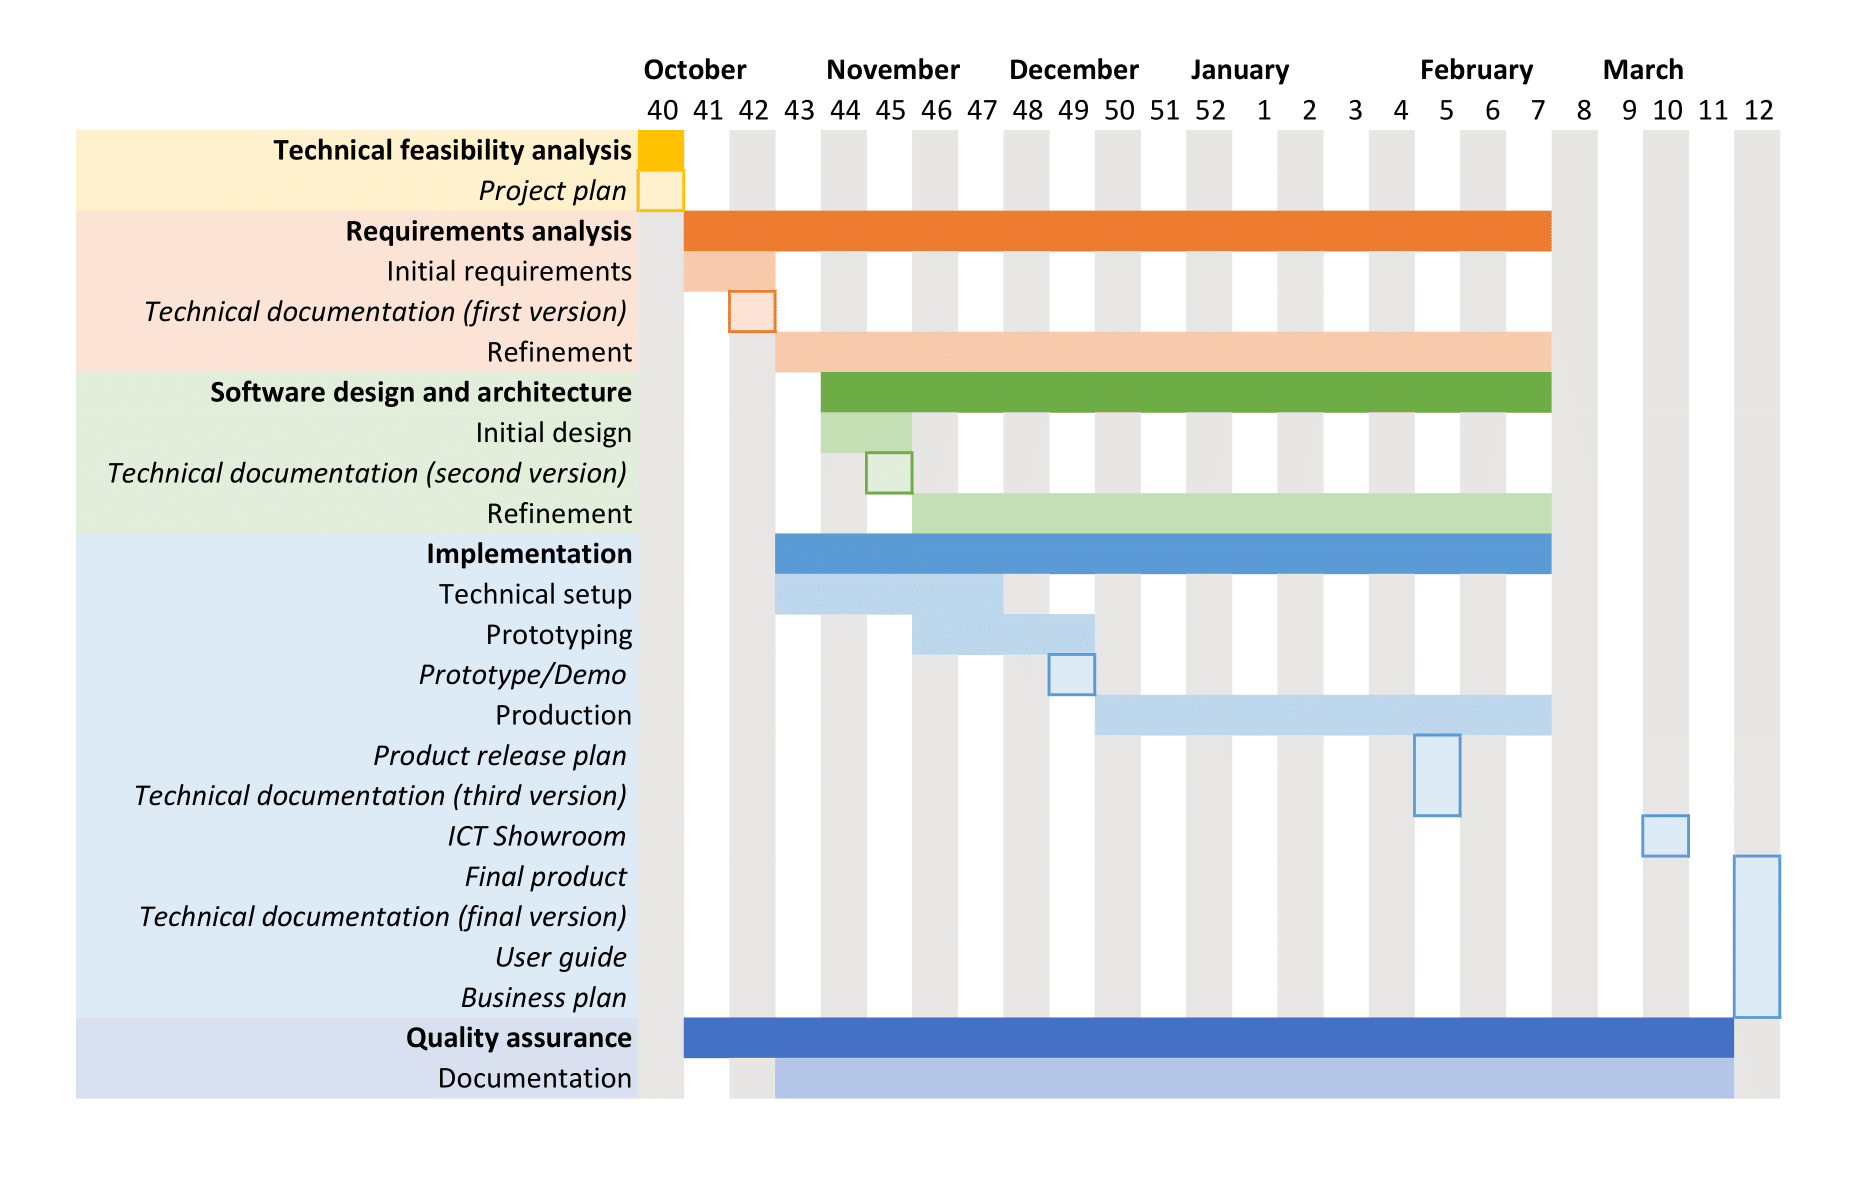
\includegraphics[width=\linewidth]{images/schedule}
	\caption{Schedule}
	\label{fig:schedule}
\end{figure}

	
	\chapter{Risks}\label{chp:risks}
	\thispagestyle{fancy}
	\begin{enumerate}[a.]
	\item Co-development of protocol and implementation. The VRGP protocol is, as of now, unfinished and will be extended and refined at the same time that we develop the VRGP implementation. Therefore, we will need to pay attention to keeping the protocol specification and implementation in sync.
	\item Work distribution. Even being rather a big team, the job to do is not only difficult, but it implies the contribution to the VRGP specification, so every developer will have to be aware of the protocol evolution even if they don’t participate directly in it. This can bring us overwork and misinformation.
	\item Deadlines. Considering that the team members are students and that carries extra work such as studies, sports, and other activities, sometimes it is difficult to guarantee that the deliveries fit into the deadlines. This risk is even bigger taking into account the previous risk, which can make us lose time.
	\item Dependency. This project is just a subproject of a bigger one, Åboat, so it depends on the physical installation in the boat and of other services.
\end{enumerate}

\noindent
In order to mitigate risks a and b, the wisest decision is to start slowly and make everyone participate in the development of the protocol. Doing this we avoid starting to implement the VRGP protocol without a solid specification and at the same time assure us that everyone knows the protocol. The disadvantage of this approach is the tight schedule it leaves for implementing the protocol.
\\\\
Risk c is half-mitigated with the previous approach to the development of the protocol implementation. There’s not much to do in order to gain time as we are students and will be during the whole time. We can only prevent it by having a good organization and a well-structured schedule.
\\\\
For risk d, in case we can’t test with the physical boat or other pieces of the architecture are unavailable, we can develop small simulation codes.

	
	\chapter{Tracking}\label{chp:tracking}
	\thispagestyle{fancy}
	\section{Project meetings}\label{sec:meetings}

We plan to have team meetings every week to plan the work for the upcoming week and review the progress of the past week as well as our overall project status and progress. These meetings do not require every team member to attend every single week. Depending on the workload in the specific weeks, the meetings can either focus on the project work or some leisure activities, or both.
\\\\
The further we move on with the project, the less discussions we expect in the meeting. As we are a large group of seven members, we want to keep the meetings almost exclusively organisational and only discuss urgent and important matters that truly concern everyone in the team. The work on the project is done in smaller groups to ensure productivity.
\\\\
In addition, we will meet with our customers once per week during the first month of the project as we have to gather a lot of information and discuss a lot of topics and decisions in the beginning. We will then switch to bi-weekly meetings afterward and finally to monthly meetings in the end as the topics under discussion will get less the more we progress with and dive into the project. Regarding certain deadlines, we will most likely have additional ad-hoc meetings with our customers to discuss e.g. the requirements. Again, these meetings do not necessarily require the attendance of all team members every time, but rather certain roles to take part. We also agreed with our customers to prepare these meetings with an agenda beforehand as required by the course.

\section{Time tracking}\label{sec:time-tracking}

For now, we created a table sheet for everyone to keep their working hours for the project per day updated. In the future, especially when we start to work on different topics, we want to integrate the time tracking into our Scrum tool framework and find a more intuitive tool for the purpose with the possibility to categorize the job types.

\end{document}
